\newpage
\section{Appendix}
The source code of this project can be found at:\\ \url{https://github.com/nickma82/advanced_multiprocessor_prog}

\begin{figure}[ht]
  \centering
\begin{tabular}{ l | c c c c }
 & add & contains & remove & mixed\\
 \hline
reference & 418.53 &  231.50 &  470.04  & 272.85\\
fine grained lock. & 17155.33 & 9360.36 & 8433.88 & 32.25 \\
optimistic sync. & 2609.88  & 418.71 & 3421.86 &   38.19\\
lazy sync. & 1333.05 &  289.80 &  215.82  &  25.22\\
lock free & 1128.28  & 161.50  & 115.61   & 29.39\\
\end{tabular}
  \caption{Average time in milliseconds of 100 throughput benchmark runs on Mars, 80 threads, each thread ran the iteration 1000 times}
  \label{mars_throughput}
\end{figure}

\begin{figure}[ht]
  \centering
\begin{tabular}{ l | c c c c }
 & add & contains & remove & mixed\\
 \hline
reference & 29.75  &  25.17  &  25.77 &   27.94 \\
fine grained lock. & 5759.07 & 6059.24 & 5886.83 & 37.72 \\
optimistic sync. & 1348.86 &  634.34 & 2344.10  &  39.79 \\
lazy sync. & 635.12  & 328.49 &  307.21  &  30.92 \\
lock free & 687.51  & 320.21 &  358.25  &  16.03\\
\end{tabular}
  \caption{Average time in milliseconds of 100 throughput benchmark runs on Ceres, 64 threads, each thread ran the iteration 1000 times}
  \label{ceres_throughput}
\end{figure}

\begin{figure}[H]
  \centering 
  \includegraphics[height=0.93\textheight]{pictures/timer_benchmarks.eps}
  \caption{average execution time of 1000 calls to different time capture methods, measured with a wrapped \textit{clock\_gettime}}
  \label{timer_benchmark}
\end{figure}

\begin{figure}[H]
  \centering 
  \includegraphics[width=0.6\textwidth, angle=270]{pictures/throughput_add.eps}
  \caption{Comparison of \texttt{add} performance, on both machines}
  \label{addthrough}
\end{figure}

\begin{figure}[H]
  \centering 
  \includegraphics[width=0.6\textwidth, angle=270]{pictures/throughput_contains.eps}
  \caption{Comparison of \texttt{contains} performance, on both machines}
  \label{containsthrough}
\end{figure}

\begin{figure}[H]
  \centering 
  \includegraphics[width=0.6\textwidth, angle=270]{pictures/throughput_remove.eps}
  \caption{Comparison of \texttt{remove} performance, on both machines}
  \label{removethrough}
\end{figure}

\begin{figure}[H]
  \centering 
  \includegraphics[width=0.6\textwidth, angle=270]{pictures/throughput_mixed.eps}
  \caption{Comparison of \texttt{mixed} performance, on both machines}
  \label{mixedthrough}
\end{figure}

\begin{figure}[H]
  \centering 
  \includegraphics[height=0.95\textheight]{pictures/mars_fairness_plot.eps}
  \caption{Histograms of 5 second runs of \texttt{insert}, on Mars, with 80 threads}
  \label{marsfairness}
\end{figure}

\begin{figure}[H]
  \centering
  \includegraphics[height=0.95\textheight]{pictures/ceres_fairness_plot.eps}
  \caption{Histograms of 5 second runs of \texttt{insert}, on Ceres, with 500 threads}
  \label{ceresfairness}
\end{figure}

\nocite{*} %add unreferenced bibliography items

\clearpage %force bibliography to the end
\bibliography{bibliography}{}
\bibliographystyle{plain}